\documentclass[12pt,aspectratio=169]{beamer}
% \hypersetup{pdfpagemode=FullScreen}

\usepackage{upgreek}
\usefonttheme{professionalfonts}

\renewcommand*{\thefootnote}{\fnsymbol{footnote}}

\mode<presentation>
\useoutertheme[subsection=false]{miniframes}

\AtBeginSection[]{
  \begin{frame}
  \centering
  \begin{beamercolorbox}[sep=8pt,center,shadow=true,rounded=true]{title}
    \usebeamerfont{title}\insertsectionhead\par%
  \end{beamercolorbox}
  \end{frame}
}

\title{Amazon SageMaker Model Parallelism: A General and Flexible Framework for Large Model Training}
\author{Can Karakus\inst{1} Rahul Huilgol\inst{1} Fei Wu\inst{1} Anirudh Subramanian\inst{1} Cade Daniel\inst{1} Derya Cavdar\inst{1} Teng Xu\inst{1}
Haohan Chen\inst{1} Arash Rahnama\inst{1} Luis Quintela\inst{1}}
\institute{\inst{1} Amazon}
\date{Presenter: Shiwei Zhang}

\begin{document}
    \beamertemplatenavigationsymbolsempty

    \makeatletter
    \def\beamer@andinst{\\[.1em]}
    \makeatother

    \begin{frame}
        \titlepage
    \end{frame}

    \section{Prelude}

    \begin{frame}
        \frametitle{Amazon SageMaker}

        \vskip 1em
        \centering
        
\includegraphics[width=0.8\textwidth]{sagemaker.png}
    \end{frame}

    \begin{frame}
        \frametitle{Content}

        \begin{itemize}
            \setlength{\itemsep}{.8em}
            \item Design Principle and Overview
            \item Pipeline Parallelism
            \item Tensor Parallelism
            \item Experiments
            \item Summary
        \end{itemize}
    \end{frame}

    \section{Design Principle and Framework Overview}

    \begin{frame}
        \frametitle{Motivation}

        Existing systems are not flexible enough to handle:
        \vskip .5em

        \begin{itemize}
            \small
            \setlength{\itemsep}{.2em}
            \item architectures that do not consist of a single transformer encoder or large non-transformer architectures,
            \item architectures that do not consist of a consecutive sequence of identical layers,
            \item a single large component in an otherwise small model,
            \item architectures that make extensive use of module/parameter re-use,
            \item scripts with conditional execution flows,
            \item and non-conventional execution patterns such as mixture-of-experts layers.
        \end{itemize}
    \end{frame}

    \begin{frame}
        \frametitle{Design Principles}

        \begin{itemize}
            \setlength{\itemsep}{.8em}
            \item Do not abstract away the training step
            \item Preserve framework features and characteristics
            \item Do not limit to specific architectures
        \end{itemize}
    \end{frame}

    \begin{frame}
        \frametitle{Framework Overview}

        \begin{columns}
            \begin{column}{0.5\textwidth}
                The library features pipeline, tensor, and data parallelism, controlled by the three groups.
                \vskip 1em
                The entry function (training loop) is wrapped in a \texttt{smp.step} decorator to activate this library.
            \end{column}
            \begin{column}{0.5\textwidth}
                \includegraphics[page=4,trim=11.5cm 17.5cm 2.2cm 2.2cm,clip,scale=0.85]{paper.pdf}
            \end{column}
        \end{columns}
    \end{frame}

    \section{Pipeline Parallelism}

    \begin{frame}
        \frametitle{Background}

        In pipeline parallelism, the model is partitioned into \textbf{stages}. Each stage is put on one device.
        Multiple microbatches are running concurrently in a pipeline.
        \vskip 1em

        \centering
        \includegraphics[page=13,trim=2.5cm 17.5cm 11.5cm 8.5cm,clip,scale=1.1]{paper.pdf}
        \includegraphics[page=13,trim=2.5cm 14.5cm 11.5cm 11.5cm,clip,scale=1.1]{paper.pdf}
    \end{frame}

    \begin{frame}
        \frametitle{Tree Structure and Message Passing Workflow}

        \begin{columns}
            \begin{column}{0.5\textwidth}
                The model is viewed as a hierarchy of modules based on PyTorch class definition.
                \vskip 1em

                Each pipeline stage runs an execution server, which is a Python thread that listens for
                incoming execution requests.
            \end{column}
            \begin{column}{0.5\textwidth}
                \includegraphics[page=5,trim=11.5cm 12.5cm 2.5cm 8.5cm,clip,scale=0.9]{paper.pdf}
            \end{column}
        \end{columns}
    \end{frame}

    \section{Partitioning Algorithm}

    \begin{frame}
        \frametitle{Problem Definition}

        For a tree $\mathcal{T} = (\mathcal{V}, \mathcal{E})$, we define $Q(n)$ as the set of children of a node
        $n \in \mathcal{V}$. A cost $c(n)$ is associated with each node $n$ representing the memory and computation cost
        of the subtree.
        \vskip 1em

        The goal of the algorithm is to find the device assignment $d(n)$ for each node $n$.
        \vskip 1em

        Virtual devices: in this part, ``device'' stands for the unit of pipeline groups, which may contain multiple
        GPUs.
        \vskip 1em

        Module Nodes: A Node in the tree $V$ may contain multiple modules if they share the same parameter. In this
        case, the edges are arbitrarily pruned to keep it a tree.
    \end{frame}

    \begin{frame}
        \frametitle{Main loop}

        \centering
        \includegraphics[page=8,trim=1.8cm 20.5cm 11.2cm 2.1cm,clip,scale=1.1]{paper.pdf}
    \end{frame}

    \begin{frame}
        \frametitle{Cost function}
        \small

        $$
            \bar{C}(m) = \alpha w(m) + (1 - \alpha)\psi(m)
        $$
        where $\bar{C}(m)$ is the unnormalized cost, $w(m)$ is the memory cost, and $\psi(m)$ is the computation cost of
        module $m$.

        \vskip 1em
        The cost of a Module Node $n$ is defined recursively as the sum of the costs of the set of modules
        $M(n)$ it contains and the costs of its children $Q(n)$
        $$
            C(n) = \sum_{m\in M(n)}\bar{C}(m) + \sum_{p\in Q(n)}C(p)
        $$

        \vskip 1em
        The final cost is normalized by the cost of the root $r$
        $$
            c(n) = \frac{C(n)}{C(r)}
        $$

    \end{frame}

    \begin{frame}
        \frametitle{Segmentation}

        To assign the set of devices $P(n)$ to each child node in $Q(n)$, we first partition the sequence of $Q(n)$ into
        $l$ segments such that
        $$
            \min_{\mathcal{P}} \omega(\mathcal{P}) = \min_{\mathcal{P}} \max_{S \in P}\sum_{p \in S}c(p)
        $$

        This can be solved with dynamic programming using the recursion:
        $$
            c(k, i) = \min_{j \leq i} \max\{ c(k-1, j), \sum_{q \in Q(n, j)} c(q) \}
        $$
        where $c(k, i)$ is the partition cost $\mathcal{P}$ achieved in partitioning the first $i$ elements of $Q(n)$
        into $k$ partitions, and $Q(n, j)$ represents the sub-sequence of $Q(n)$ from element $j$ onwards.

    \end{frame}

    \begin{frame}
        \frametitle{Device Allocation}

        \centering
        \includegraphics[page=15,trim=1.8cm 21cm 11.2cm 2.1cm,clip,scale=1.1]{paper.pdf}
    \end{frame}

    \begin{frame}
        \frametitle{Recursive partitioning}

        At the end of D'Hondt allocation, there are three possible scenarios for each segment:

        \begin{itemize}
            \item No device is assigned to it. This segment will be put on the same device as the parent node.
            \item One device is assigned to the segment. The segment and all its subtrees will be placed on the device.
            \item Multiple devices are assigned to the segment. If this segment has only one node, all devices are
            assigned to it (it will be revisited in Algorithm 1). Otherwise, the segment is further divided into smaller
            segments recursively.
        \end{itemize}
    \end{frame}

    \begin{frame}
        \frametitle{Example Partitioning}

        Auto-partition decision over T5-11B with $\alpha = 1.0$
        \vskip 1em

        \centering
        \includegraphics[page=16,trim=2.7cm 20.5cm 3cm 2.1cm,clip,scale=0.88]{paper.pdf}
    \end{frame}

    \begin{frame}
        \frametitle{Another Example Partitioning}

        Auto-partition decision over T5-11B with $\alpha = 0.2$
        \vskip 1em

        \centering
        \includegraphics[page=17,trim=2.7cm 20.5cm 3cm 2.1cm,clip,scale=0.88]{paper.pdf}
    \end{frame}

    \section{Tensor Parallelism}

    \begin{frame}
        \frametitle{Tensor Parallelism}

        SageMaker achieves tensor parallelism by providing drop-in replacement layers like \texttt{DistributedLiner},
        \texttt{DistributedEmbedding}, \texttt{DistributedTransformer}, etc.
        \vskip 1.5em

        \centering
        \includegraphics[page=9,trim=1.9cm 22.5cm 11.5cm 2.3cm,clip,scale=]{paper.pdf}
    \end{frame}

    \section{Experiments}

    \begin{frame}
        \frametitle{10-billion parameter RoBERTa and BERT}

        \begin{itemize}
            \setlength{\itemsep}{.5em}
            \item Hardware: 16 nodes, each equipped with 8 A100.
            \item Models: RoBERTa/BERT, 10B parameters
            \item Baselines: DeepSpeed with ZeRO stage 2
        \end{itemize}
        \vskip 1em

        \centering
        \includegraphics[page=10,trim=11.2cm 22.5cm 2.8cm 3.35cm,clip,scale=1]{paper.pdf}
    \end{frame}

    \begin{frame}
        \frametitle{175-billion parameter GPT-3}

        A GPT-3 model with 175-billion parameters and a sequence length of 2048 is trained on 120 nodes for a total of
        960 A100 GPUs. The pipeline parallelism degree is 6 and tensor parallelism degree is 8.
    \end{frame}

    \begin{frame}
        \frametitle{Neural collaborative filtering}

        \begin{columns}
            \begin{column}{0.5\textwidth}
                \begin{itemize}
                    \setlength{\itemsep}{.5em}
                    \item Hardware: 4 nodes, each equipped with 8 A100.
                    \item Model: NCF
                    \item Baseline: Pure tensor-parallelism
                \end{itemize}
                \vskip 1em

                \centering
                \includegraphics[page=10,trim=12cm 3cm 3cm 22.75cm,clip,scale=1]{paper.pdf}
            \end{column}
            \begin{column}{0.5\textwidth}
                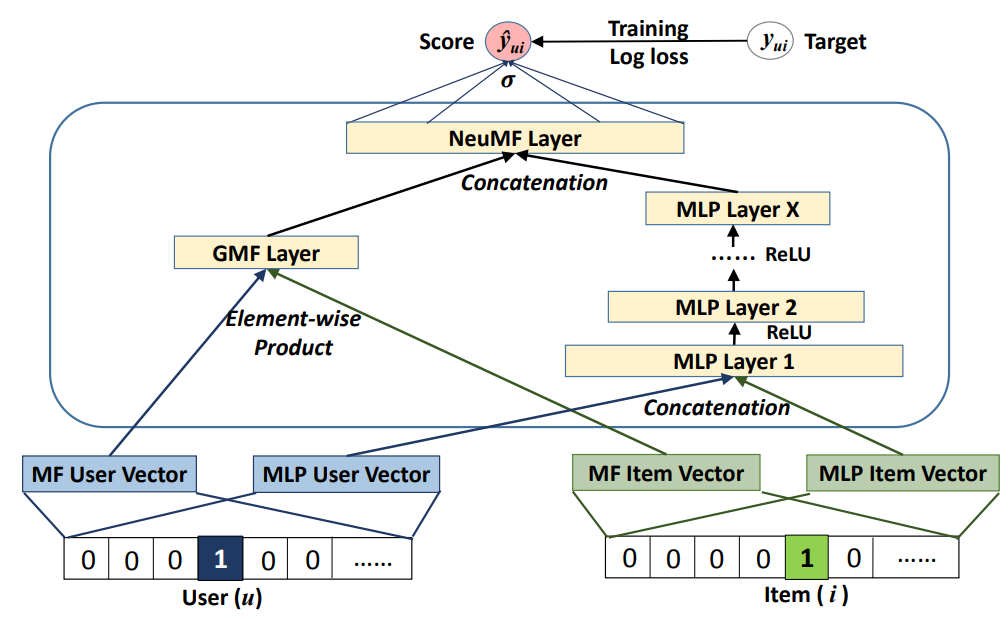
\includegraphics[width=\textwidth]{ncf.png}
            \end{column}
        \end{columns}
    \end{frame}

    \section{Summary}

    \begin{frame}
        \frametitle{Conclusion}

        \textbf{Strength}

        \vskip .6em
        \begin{itemize}
            \setlength{\itemsep}{.8em}
            \item Tree structure and message passing workflow.
            \item Automatic pipeline parallelism based on dynamic programming and D'Hondt method.
        \end{itemize}

        \vskip 1em
        \textbf{Limitation}

        \vskip .6em
        \begin{itemize}
            \setlength{\itemsep}{.8em}
            \item The proposed methods do not solve the problems listed in motivation.
            \item The experiment results are not very good.
            \item There is no analysis (optimality, complexity, etc.) for the proposed methods.
        \end{itemize}
    \end{frame}

    \begin{frame}
        \frametitle{Takeaways}

        \begin{itemize}
            \setlength{\itemsep}{.8em}
            \item In addition to the linearly-connected layers and DAG structures, we can also view a model as a tree.
            \item The message-passing architecture may provide new challenges and opportunities.
        \end{itemize}
    \end{frame}

    \appendix

    \begin{frame}
        \vskip 1em

        \centering \huge
        Thank you!
    \end{frame}
\end{document}
